\newpage
\chapter*{Riassunto}

\addcontentsline{toc}{chapter}{Riassunto}

L'apprendimento profondo per rinforzo (in inglese \textit{deep reinforcement 
learning} - DRL) ha recentemente suscitato un grande interesse nel campo 
dell'intelligenza artificiale, per la sua capacit\`a senza precedenti nel 
risolvere problemi di controllo considerati fino ad ora inavvicinabili.
A partire dalla pubblicazione dell'algoritmo \textit{deep Q-learning} (DQN) di 
Mnih et al.\ \cite{mnih2015human}, il campo dell'apprendimento per rinforzo ha 
vissuto un vero e proprio rinascimento, caratterizzato da un susseguirsi di 
pubblicazioni con algoritmi di controllo sempre pi\`u efficaci nel risolvere 
ambienti ad alta dimensionalit\`a, con prestazioni simili o superiori agli esseri 
umani. 
Tuttavia, una caratteristica comune agli algoritmi di DRL \`e la 
necessit\`a di utilizzare un enorme numero di campioni di addestramento per
arrivare a convergenza. Alcune delle pubblicazioni pi\`u recenti cercano di 
affrontare la problematica, riuscendo per\`o ad abbassare questo numero al 
massimo di un ordine di grandezza.

Lo scopo di questa tesi \`e presentare un algoritmo di DRL che riesca ad 
apprendere politiche di controllo soddisfacenti in ambienti complessi, 
utilizzando solo una frazione dei campioni necessari agli algoritmi dello stato 
dell'arte. 
Il nostro agente utilizza l'apprendimento profondo non supervisionato per 
estrarre una rappresentazione astratta dell'ambiente, e l'apprendimento per 
rinforzo in modalit\`a \textit{batch} per ricavare una politica di controllo 
a partire da questo nuovo spazio degli stati. 
Aggiungiamo, inoltre, una procedura di selezione delle \textit{feature} 
applicata alla rappresentazione estratta dall'ambiente, in modo da ridurre al 
minimo i requisiti computazionali del nostro agente. 

In fase sperimentale, applichiamo il nostro algoritmo ad alcuni ambienti di test 
dei sopracitati giochi Atari, confrontandolo con le prestazioni di DQN. 
Come risultato principale, mostriamo che il nostro agente \`e in grado di 
raggiungere in media un quarto dei punteggi ottenuti da DQN sugli stessi 
ambienti, ma utilizzando circa un centesimo dei campioni di addestramento.
Mostriamo inoltre che, a parit\`a di campioni raccolti dal nostro algoritmo per
raggiungere le migliori prestazioni, i punteggi ottenuti dal nostro agente sono 
in media otto volte pi\`u alti di quelli di DQN. 

\section*{Apprendimento Profondo}
%
\begin{figure}[t]
    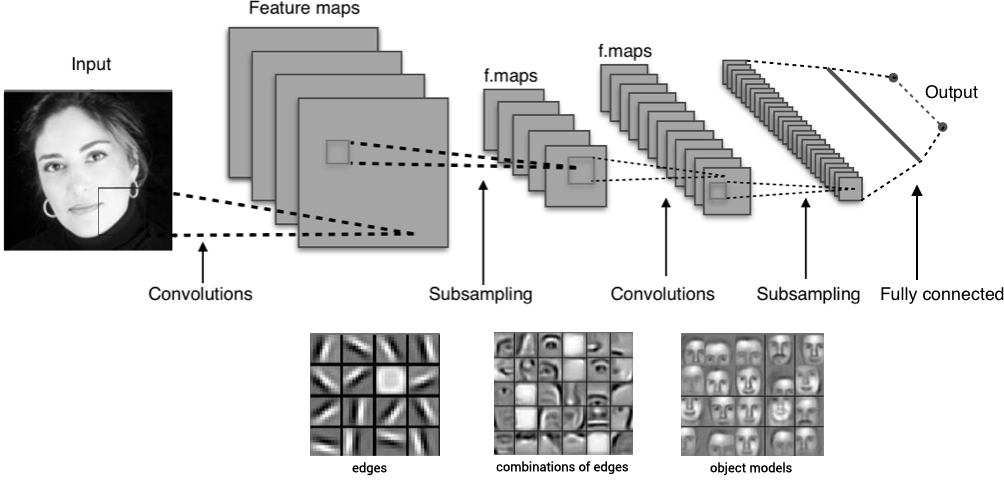
\includegraphics[width=\textwidth]{pictures/abs_cnn}
    \centering
    \caption[Esempio di estrazione di feature con una CNN]{Esempio
	    di estrazione gerarchica di feature con una CNN.}
    \label{f:abs_cnn}
\end{figure}
%
L'apprendimento profondo (normalmente noto con il termine inglese 
\textit{deep learning}) \`e una tecnica di apprendimento automatico utilizzata
per estrarre rappresentazioni astratte del dominio. 
I metodi profondi si basano su molteplici livelli di rappresentazione,
ottenuti dalla composizione di moduli semplici, ma non lineari, che trasformano 
la rappresentazione ricevuta in ingresso in una rappresentazione leggermente 
pi\`u astratta. 

Il deep learning \`e alla base della ricerca moderna in 
apprendimento automatico, ed i risultati pi\`u impressionanti sono stati 
tipicamente raggiunti grazie alla versatilit\`a delle reti neurali.
Oltre ad essere un potente approssimatore universale, questo semplice modello 
ispirato alla struttura interconnessa del cervello animale si presta alla 
composizione gerarchica, rendendolo un blocco ideale per l'apprendimento 
profondo.
Gran parte dei progressi nel campo del deep learning sono dovuti alle reti 
neurali convoluzionali (in inglese \textit{convolutional neural networks} - CNN), 
ispirate al funzionamento della corteccia visiva del cervello (Figura \ref{f:abs_cnn}). 
Le CNN sono state applicate con notevole successo a svariati problemi, dalla 
visione artificiale \cite{krizhevsky2012imagenet, szegedy2015going} alla 
traduzione automatica \cite{wu2016google}, e si basano sull'utilizzo di 
\textit{filtri} che vengono fatti scorrere sull'ingresso ad ogni livello, per 
individuare correlazioni spaziali locali che caratterizzino il dominio. 
L'efficacia delle CNN deriva proprio da questa natura intrinsecamente spaziale, 
che consente di processare domini complessi (come le immagini) con un'ottima 
generalit\`a.

\section*{Deep Reinforcement Learning}
Il deep reinforcement learning (DRL) \`e una branca dell'apprendimento 
per rinforzo che utilizza approssimatori ad apprendimento profondo per
estrarre una rappresentazione astratta dell'ambiente, e utilizza poi questa
rappresentazione per apprendere una politica di controllo ottimale.
Il DRL ha causato una vera e propria rivoluzione nel campo dell'intelligenza 
artificiale, e la letteratura sulla materia ha visto un incremento esponenziale
delle pubblicazioni.
Tra queste, citiamo nuovamente l'algoritmo che ha innescato l'interesse nel DRL, 
DQN di Mnih et al.\ \cite{mnih2015human}, e i derivati di DQN proposti da Van 
Hasselt et al.\ (2016) \cite{van2016deep} con \textit{Double DQN} (DDQN), Schaul 
et al.\ (2016) \cite{schaul2016prioritized} con \textit{prioritized experience 
replay} e Wang et al.\ (2016) \cite{wang2016dueling} con 
\textit{dueling architecture}. 
Altri approcci proposti nella letteratura di DRL includono l'algoritmo 
\textit{Asynchronous Advantage Actor-Critic} (A3C) di Mnih et al.\ (2016) 
\cite{mnih2016asynchronous} caratterizzato da un'ottima velocit\`a di 
apprendimento, il programma \textit{AlphaGo} di Silver et al.\ (2016) 
\cite{silver2016mastering} in grado di sconfiggere il campione del mondo Ke Jie
nel complicato gioco da tavolo del \textit{Go}, e \textit{Neural Episodic 
Control} di Pritzel et al.\ (2017) \cite{pritzel2017neural}, che al momento
della stesura di questa tesi costituisce lo stato dell'arte per l'apprendimento 
sui famosi ambienti \textit{Atari games}.

La tipica applicazione del DRL consiste nel risolvere problemi di controllo a 
partire dalla rappresentazione visiva dell'ambiente. Questa configurazione 
consente di sfruttare l'enorme capacit\`a descrittiva delle CNN e permette di 
affrontare problemi complessi senza la necessit\`a di ingegnerizzare i
descrittori dell'ambiente. 

\section*{Feature Profonde per l'Apprendimento Efficiente}
Come argomento centrale di questa tesi presentiamo un algoritmo di deep 
reinforcement learning che combina:
\begin{itemize}
    \item l'apprendimento profondo non supervisionato per estrarre una 
    rappresentazione dell'ambiente;
    \item un algoritmo per la selezione di feature orientato al controllo, per
    ridurre al minimo i requisiti computazionali dell'agente;
    \item un algoritmo di apprendimento automatico in modalit\`a \textit{batch}, 
    per apprendere una politica a partire dalla rappresentazione prodotta dagli 
    altri due moduli.
\end{itemize}
Lo scopo principale della procedura presentata \`e quello di apprendere una
politica di controllo efficace su un ambiente complesso, utilizzando il minor
numero possibile di campioni di addestramento. 

Per l'estrazione di feature dall'ambiente, utilizziamo un \textit{autoencoder} 
convoluzionale (AE).
L'AE \`e una forma di rete neurale che viene utilizzata per apprendere una 
rappresentazione del dominio in maniera non supervisionata, costituita da due 
moduli separati: un \textit{encoder} e un \textit{decoder}.
Lo scopo dell'encoder \`e semplicemente quello di estrarre una rappresentazione
compressa degli ingressi, mentre quello del decoder \`e di invertire questa
trasformazione e ricostruire l'ingresso originale a partire dalla compressione 
prodotta dall'encoder. 
I due componenti vengono addestrati come un'unica rete neurale, propagando il 
gradiente su tutti i pesi contemporaneamente. 
Al termine dell'apprendimento, l'encoder viene utilizzato per comprimere gli 
elementi del dominio, idealmente implementando una forma di compressione senza 
perdita che riduca la dimensionalit\`a dello spazio di ingresso. 
Identifichiamo questa compressione come la trasformazione $ENC: S \rightarrow \tilde{S}$, 
dallo spazio degli stati originali $S$, allo spazio delle feature astratte $\tilde{S}$.
%
\begin{figure}
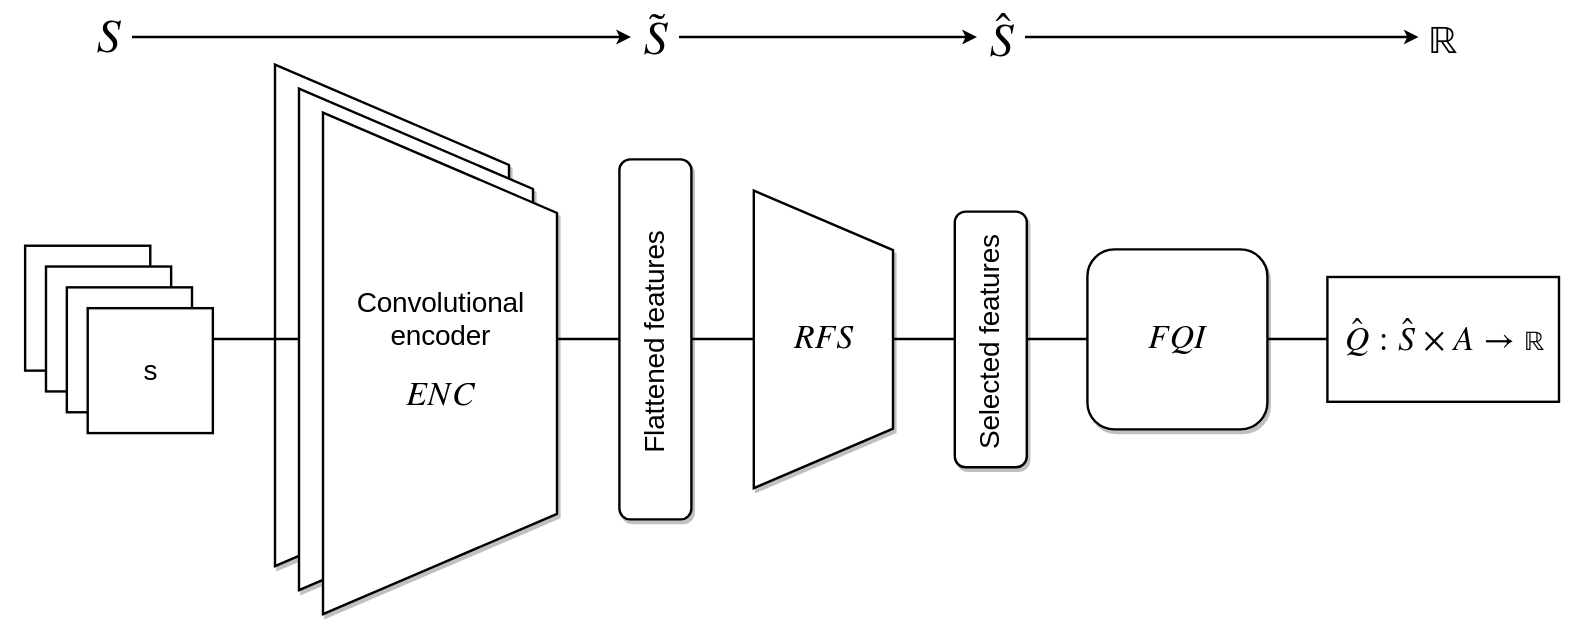
\includegraphics[width=\textwidth]{pictures/full_pipeline}
\centering
\caption[Rappresentazione dei tre moduli principali]{Rappresentazione
						     schematica della composizione dei tre moduli, con le rispettive
						     trasformazioni evidenziate in alto.}
\label{f:abs_full}
\end{figure}
%

Il secondo modulo della nostra catena di addestramento \`e l'algoritmo 
\textit{Recursive Feature Selection} di Castelletti et al.\ \cite{castelletti2011tree}.
Questa procedura di selezione delle feature utilizza l'apprendimento supervisionato
per ordinare le feature di stato di un ambiente in base alla loro utlit\`a per 
il controllo, e riduce la dimensionalit\`a del dominio rimuovendo le feature 
meno utili a questo fine. 
Nel nostro caso, utilizziamo una versione di RFS basata sugli alberi decisionali
per ridurre ulteriormente la rappresentazione estratta dall'AE, in modo da 
ottenere uno spazio delle feature minimale ed essenziale per il controllo. 
Anche in questo caso, il prodotto del modulo \`e una trasformazione 
$RFS: \tilde{S} \rightarrow \hat{S}$, dove $\hat{S}$ identifica lo spazio 
ridotto. 

Infine, utilizziamo l'algoritmo di apprendimento automatico batch 
\textit{Fitted Q-Iteration} (FQI) \cite{ernst2005tree} per apprendere una 
politica  di controllo per l'ambiente a partire da una raccolta di transizioni 
$(s, a, r, s')$ (\textit{stato, azione, rinforzo, stato prossimo}) dove 
$s, s' \in \hat{S}$. Alla fine dell'addestramento, l'algoritmo produce un 
approssimatore della funzione di valore di azione $\hat{Q}: \hat{S} \times A \rightarrow \mathbb{R}$, 
dove $A$ \`e lo spazio delle azioni. 

I tre moduli vengono addestrati in sequenza per produrre le rispettive 
trasformazioni, e alla fine della fase di addestramento vengono combinati 
per poter utilizzare la funzione $\hat{Q}$ prodotta da FQI a partire dallo
spazio degli stati originale (Figura \ref{f:abs_full}).
La sequenza di addestramento, poi, viene ripetuta all'interno
di un ciclo principale, che sequenzialmente raccoglie un insieme di campioni
su cui addestrare i tre moduli, utilizzando una politica a tasso di esplorazione
decrescente in modo da sfruttare sempre di pi\`u la conoscenza appresa 
dall'agente, fino a convergenza. Ogni sequenza di addestramento \`e seguita
da una fase di valutazione, per stabilire se le prestazioni dell'agente siano
soddisfacenti ed eventualmente terminare la procedura. 

\section*{Esperimenti e Conclusioni}
Nella fase sperimentale applichiamo l'algoritmo a tre ambienti dei giochi Atari,
e per valutare le prestazioni del nostro agente le compariamo a quelle ottenute
da DQN di Mnih et al.\ \cite{mnih2015human} sugli stessi giochi.

Osserviamo che l'AE riesce ad ottenere un'ottima precisione nella ricostruzione 
dello spazio originale degli stati, e che le feature estratte dall'encoder 
sono sufficientemente astratte.
Per verificare la bont\`a delle feature al fine del controllo, addestriamo un 
modello supervisionato per approssimare la funzione $Q$ appresa da DQN, a 
partire dalle feature prodotte dall'AE. 
L'alto coefficiente di correlazione dei valori predetti in validazione conferma 
che le feature estratte sono adatte al controllo, o che quantomeno contengono 
tutta l'informazione necessaria a stimare le funzioni di valore ottime 
dell'ambiente. 

A causa degli enormi requisiti di potenza computazionale, possiamo 
condurre pochi esperimenti relativi a RFS, e siamo costretti a rimuoverlo 
completamente dalla catena di addestramento per valutare le prestazioni
finali dell'agente in tempi trattabili. 
I tre esperimenti che portiamo a termine (uno per ogni ambiente), producono 
risultati variabili e inaspettati, e ci portano a rimandare l'analisi della
procedura di selezione ad un secondo momento. 

Infine, la valutazione dell'algoritmo completo conferma il raggiungimento 
dell'obiettivo di efficienza e sottolinea un grande potenziale della procedura,
che tuttavia non riesce ad arrivare alle stesse prestazioni dello stato 
dell'arte.
Il nostro agente riesce ad ottenere in media il $25\%$ del punteggio di DQN, 
utilizzando per\`o lo $0.4\%$ dei campioni di addestramento richiesti in media
da DQN per raggiungere la miglior prestazione. 
Allo stesso tempo, valutando i punteggi raggiunti da entrambi gli algoritmi 
limitandosi a questo numero di campioni estremamente ridotto, osserviamo che
il nostro agente ottiene punteggi mediamente superiori di otto volte rispetto a 
quelli di DQN, che necessita di un numero dieci volte pi\`u grande di esempi 
per imparare una politica equivalente.
Il nostro algoritmo dimostra dunque una grande efficienza nell'utilizzo dei 
campioni, rendendolo adatto al controllo in situazioni in cui la raccolta
di campioni \`e difficile o costosa. 


































